\IEEEraisesectionheading{\section{简介}
\label{sec:introduction}}

在计算机视觉众多的技术领域中,目标检测(Object Detection)也是一项非常基础的任务,图像分割、物体追踪、关键点检测等通常都要依赖于目标检测。在目标检测时,由于每张图像中物体的数量、大小及姿态各有不同,也就是非结构化的输出,这是与图像分类非常不同的一点,并且物体时常会有遮挡截断,所以物体检测技术也极富挑战性,从诞生以来始终是研究学者最为关注的焦点领域之一。

在计算机视觉中,图像分类、目标检测和图像分割都属于最基础、也是目前发展最为迅速的3个领域,如图 \ref{fig:cv_task} 所示,这几个任务之间的区别为:

\begin{itemize}
	\item 图像分类:输入图像往往仅包含一个物体,目的是判断每张图像是什么物体,是图像级别的任务,相对简单,发展也最快。
	\item 目标检测:输入图像中往往有很多物体,目的是判断出物体出现的位置与类别,是计算机视觉中非常核心的一个任务。
	\item 图像分割:输入与物体检测类似,但是要判断出每一个像素属于哪一个类别,属于像素级的分类。图像分割与物体检测任务之间有很多联系,模型也可以相互借鉴。
\end{itemize}

在利用深度学习做物体检测之前,传统算法对于目标检测通常分为3个阶段:区域选取、特征提取和体征分类。首先选取图像中可能出现物体的位置,由于物体位置、大小都不固定,因此传统算法通常使用滑动窗口(Sliding Windows)算法,但这种算法会存在大量的冗余框,并且计算复杂度高。在得到物体位置后,通常使用人工精心设计的提取器进行特征提取,如 SIFT 和 HOG 等。由于提取器包含的参数较少,并且人工设计的鲁棒性较低,因此特征提取的质量并不高。最后,对上一步得到的特征进行分类,通常使用如SVM、AdaBoost的分类器。

\begin{figure}[!ht]
  \centering
  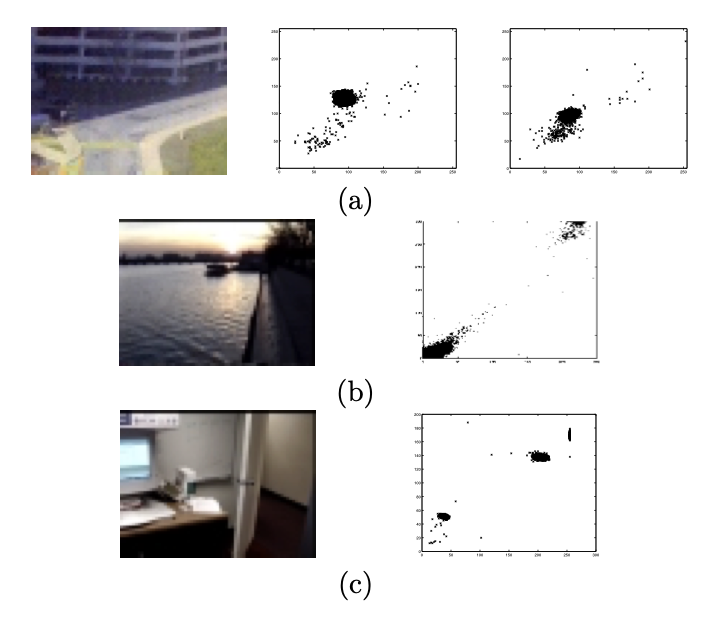
\includegraphics[width=\linewidth]{fig1}
  \caption{计算机视觉中的图像分类、目标检测和图像分割任务示意图}
  \label{fig:cv_task}
  \vspace{-0.5cm}
\end{figure}

基于深度学习的目标检测方法逐渐使目标检测进入到快速发展的阶段,比较流行的算法可以分为两类,一类是基于 Region Proposal 的R-CNN系算法(RCNN、SPPNet、FasterRCNN、Pyramid NetWorks等),它们是two-stage的,需要先算法产生目标候选框,也就是目标位置,然后再对候选框做分类与回归。而另一类是 Yolo,SSD 这类 one-stage 算法,其仅仅使用一个卷积神经网络直接预测不同目标的类别与位置。第一类方法是准确度高一些,但是速度慢,但是第二类算法是速度快,但是准确性要低一些。

本文分别利用传统的基于滑窗的目标检测算法(即机器学习方法)实现静态场景下的侧视车辆检测和基于深度学习的目标检测模型对口罩进行检测。本文剩余部分将对传统目标检测放法的原理和采用的深度学习模型的架构、实现及实验进行介绍,所有实验涉及的方法、函数实现均基于 Python 语言,其中深度学习模型的实现及训练等采用了开源深度学习框架 PyTorch。